% ------------------------------------------------------------------------------------------- %
%                                         Metodologia                                         %
% ------------------------------------------------------------------------------------------- %
\chapter{Materiais e Métodos}\label{cap:materialemetodos}

\section{Materiais}\label{sec:materiais}

\subsection{PostgreSQL}\label{subsec:postgresql}

O PostgreSQL é um banco de dados relacional contributivo, ou seja, tem seu desenvolvimento em código aberto, o que garante mais liberdade no uso, além de permitir diferentes implementações de acordo com as necessidades, e ele utiliza a linguagem SQL como base \cite{Amazon}. Muitos dos contribuintes são voluntários, mas o projeto se sustenta com patrocínios de diversas empresas de todo o mundo. É um projeto da Universidade da Califórnia em Berkeley e tem mais de 35 anos de desenvolvimento ativo na plataforma central \cite{PostgreSQL}.

\subsection{Linguagem C{\#} {\&} .NET Framework}\label{subsec:csharp}

C{\#} é uma linguagem de programação, fortemente tipada e orientada a objetos desenvolvida pela Microsoft em julho de 2000 e sua sintaxe foi baseada no C++, porém contendo influências de outras linguagens como Java. A linguagem permite que desenvolvedores construam diversos tipos de aplicações de forma segura e robusta que são executadas sobre a plataforma .NET \cite{CSharp}.

.NET Framework é uma plataforma de desenvolvimento que possui um \gls{clr}, que gerencia a execução de código. Possui também uma \gls{bcl}, oferecendo um amplo leque de classes para a construção de aplicações. A Microsoft, sua desenvolvedora, modelou a ferramenta para uso multi-plataforma, porém a ferramenta funciona melhor com o sistema operacional Windows \cite{CSharpDevelopment}.

\subsection{Python}\label{subsec:python}

Criada em 1991 por Guido van Rossum, Python é uma linguagem de programação de alto nível, interpretada e orientada a objetos com semâmtica dinâmica. Devido sua simplicidade e tipagem dinâmica, Python é uma das linguagens mais populares da atualidade, permitindo o desenvolvimento rápido de aplicações e custo reduzido de manutenção. \cite{VanRossum2009}.

Python se destaca principalmente no suporte ao desenvolvimento de aplicações voltadas a análise de dados, aprendizado de máquina e inteligência artificial, oferencendo uma ampla gama de pacotes que auxiliam na criação destas aplicações, como por exemplo, Transformers, utilizada neste projeto, NTLK, TensorFlow, PyTorch, entre outros.

\subsection{Flutter {\&} Dart}\label{subsec:flutterdart}

Flutter é um framework de desenvolvimento em código aberto, criado e disponibilizado pelo Google. Com apenas um código, é possível construir aplicativos em multi-plataformas (Android/iOS), utilizando componentes nativos de cada plataforma \cite{Flutter}. A estrutura utiliza a linguagem Dart, assíncrona e muito semelhante à linguagem JavaScript \cite{Dart}.

\subsection{Docker}\label{subsec:docker}

Docker é um motor de código aberto que automatiza a implementação de aplicações dentro de contêineres. Esta ferramenta permite a criação de aplicações mais portáteis, de fácil construção e colaboração, reduzindo o tempo em que um código escrito seja testado, implementado e utilizado \cite{TheDockerBook}.

\subsection{GPT}\label{subsec:gpt}

O \gls{gpt} é uma classe de modelos de linguagem desenvolvidos pela OpenAI, introduzido inicialmente em 2018, com base na arquitetura de transformadores. Ao longo de suas versões (GPT-1, GPT-2, GPT-3), o modelo evoluiu significativamente em capacidade e complexidade, culminando em sistemas com níveis de fluidez e coerência comparáveis ao humano.

O modelo utiliza pré-treinamento autoregressivo unidirecional, prevendo a próxima palavra em uma sequência textual considerando apenas os elementos anteriores. O treinamento do GPT utiliza aprendizado auto-supervisionado, eliminando a necessidade de anotações dos dados. \cite{Brown2020}.

Entre as características que diferenciam o GPT de outras abordagens, destaca-se sua capacidade de realizar tarefas em cenários de aprendizado de poucos ou nenhum exemplo (few-shot e zero-shot learning), particularmente com o GPT-3, que possui 175 bilhões de parâmetros, permitindo que o modelo entenda e execute instruções com base em descrições mínimas. \cite{Brown2020}.

\subsection{BERT}\label{subsec:bert}

O \gls{bert} é um modelo de linguagem baseado em transformadores desenvolvido pelo Google AI em 2018 e que revolucionou o campo do processamento de linguagem natural ao introduzir um treinamento bidirecional profundo, permitindo a captura de contextos linguísticos em ambas as direções (esquerda para direita e direita para esquerda) simultaneamente. \cite{Devlin2018}.

O treinamento bidirecional do \gls{bert} é alcançado por meio de duas técnicas, sendo elas \gls{mlm} e \gls{nsp}. \gls{mlm} mascara parte das palavras em uma frase e então o modelo é treinado para prever essas palavras com base no contexto ao redor, tanto antes quanto depois da posição mascarada. \gls{nsp} treina o modelo para determinar se uma frase B segue imediatamente uma frase A no texto, melhorando a compreensão em relação às relações entre sentenças. \cite{Devlin2018}.

As principais caracteristicas do \gls{bert} são sua bidirecionalidade e escalabilidade, sendo uma de suas versões, o BERT-Large, composto por 24 camadas, 1024 dimensões e 340 milhões de parâmetros. A partir de seu lançamento, o BERT tornou-se base para diversos avanços e está presente em aplicações práticas, como por exemplo o sistemas de busca do Google. \cite{Devlin2018}.

\subsection{BERTimbau}\label{subsec:bertimbau}

BERTimbau é um modelo de linguagem treinado a partir do \gls{bert} com o objetivo de melhorar o desempenho em tarefas de processamento de linguagem natural para o português brasileiro. O modelo representa o estado da arte em tarefas como similaridade textual em sentenças e reconhecimento de entidades nomeadas, superando o desempenho de modelos multilinguísticos. \cite{souza2020bertimbau}.

O modelo foi treinado utilizando a técnica de transferência de aprendizado (Transfer Learning), onde um modelo préviamente treinado utilizando uma grande quantidade de dados é ajustado finamente para uma tarefa similiar, retendo partes do conhecimento adquirido no treinamento original. Essa técnica reduz a quantidade de dados anotados necessários para um treinamento supervisionado e melhora o desempenho do modelo. \cite{souza2020bertimbau}.

\subsection{Azure AI Language}\label{subsec:azure}

O Azure AI Language é um serviço em nuvem de processamento de linguagem natural criado pela Microsoft que oferece a desenvolvedores ferramentas para a criação de aplicações capazes de compreender e processar a linguagem humana de forma eficiente. O serviço oferece funcionalidades como extração de palavras-chave, análise de sentimentos, reconhecimento de entidades nomeadas, sumarização de textos e entre outras. Alguns destes serviços são customizáveis, habilitando o treinamento dos modelos com dados específicos, permitindo a criação de modelos adaptados ao conjunto de dados do usuário. \cite{AzureAILanguage}.  

\subsection{Amazon Comprenhend}\label{subsec:comprehend}

O Amazon Comprehend é um serviço de processamento de linguagem natural parte da plataforma de serviços em nuvem da Amazon Web Services (AWS). O serviço extrai percepeções sobre o conteúdo de textos e documentos através de reconhecimento de entidades, extração de palavras-chave, análise de sentimentos, entre outras funcionalidades. \cite{AmazonComprehend}.

\subsection{YAKE}\label{subsec:yake}

\gls{yake} é um algoritmo de extração de palavras-chave em textos e documentos que utiliza uma abordagem não supervisionada e técnicas linguísticas e estatísticas ao invés de treinamento supervisionado para extração de informações relevantes, utilizando apenas informações presentes no texto ou documento sem a necessidade de conhecimento externo, o que torna o algoritmo agnóstico à linguagem, independente de domínio e altamente eficiente com baixo custo computacional, ao contrário de abordagens baseadas e treinamento supervisionado, como o \gls{bert} e \gls{gpt}. \cite{YakeKeywordExtractor}.

O algoritmo é composto por seis etapas principais, sendo elas, pré-processamento do texto, extração de recursos, pontuação de termos individuais geração de lista de palavras-chave candidatas, deduplicação dos dados e ranqueamento. Após a aplicação destas etapas, o algoritmo retorna uma lista de palavras-chave e uma pontuação para cada uma delas, ordenadas de acordo com sua relevância ao contexto do texto ou documento. \cite{YakeKeywordExtractor}.

\section{Métodos}\label{sec:metodo}

O presente projeto foi subdividido no desenvolvimento de três módulos principais, sendo eles, a implementação de uma \gls{api} \gls{rest} de aplicação, uma \gls{api} \gls{rest} de linguagem e uma aplicação mobile/web. Nesta seção são detalhados os métodos utilizados e os objetivos que cada módulo visa atender. 

\subsection{API de Aplicação}\label{subsec:app_api}

A \gls{api} de aplicação foi construída utilizando a linguagem C{\#} e o framework .NET. Esta \gls{api} é responsável por recepcionar, processar e responder a requisições \gls{http} realizadas pela aplicação de interface com o usuário, bem como realizar as requisições de análise linguísticas à \gls{api} de linguagem.

Dividida em cinco subdomínios e expondo quinze rotas, a \gls{api} realiza operações de autenticação, cadastro e consulta de dois tipos usuários, laboratórios e empresas, bem como a criação e atualização de demandas criadas por empresas. As requisições de extração de palavras-chave e análises semânticas são engatilhadas na criação de um perfil de usuário do tipo laboratório e na criação e atuliazação de demandas por usuários do tipo empresa. Por fim, a \gls{api} de aplicação também é responsável pela persistência das informações em uma base de dados PostgreSQL. O diagrama da figura \ref{fig:api_aplicacao} apresenta seu funcionamento básico.

\begin{figure}[htb]
    \caption{Diagrama da API de Aplicação}
    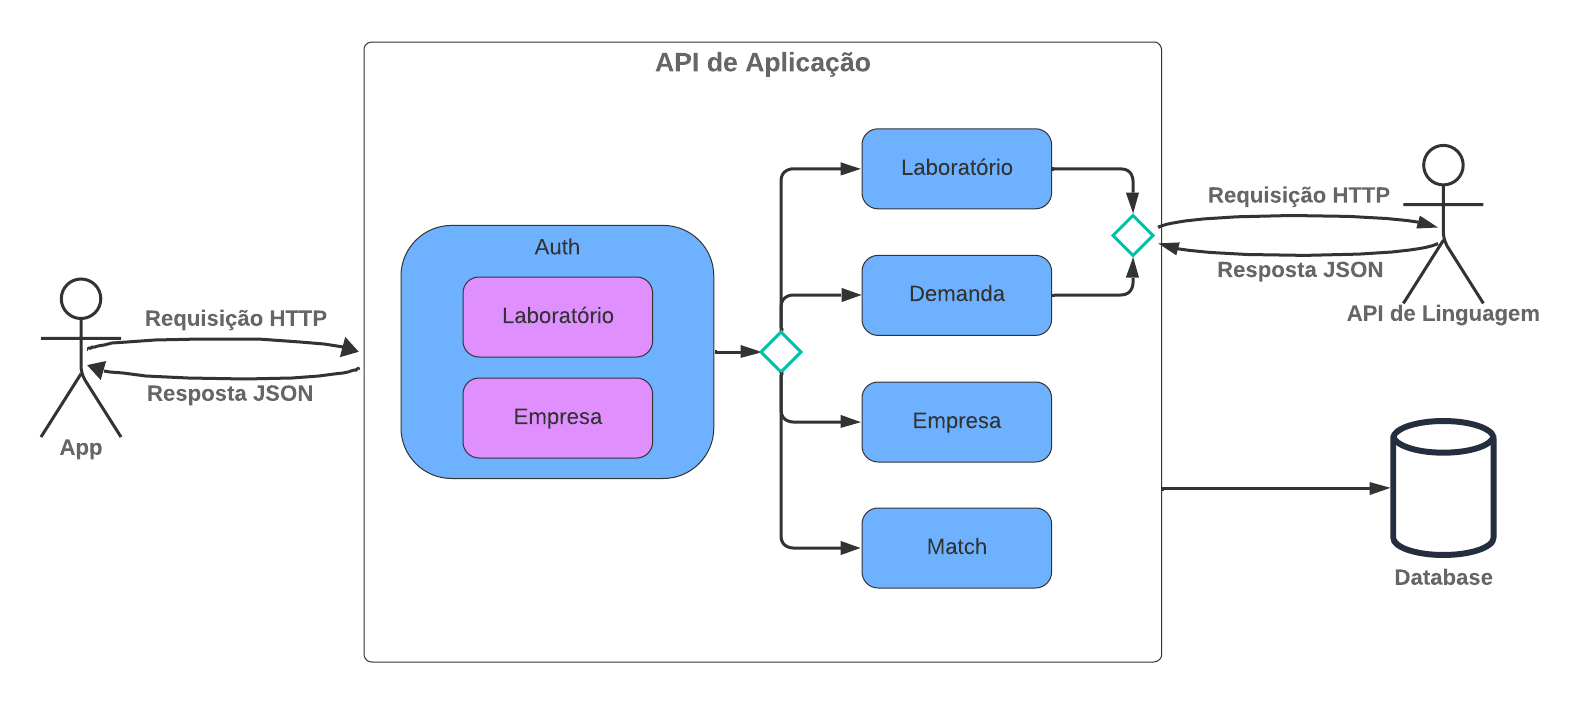
\includegraphics[scale=0.65]{api-aplicacao}
    \fonte{Autoria própria (2025)}
    \label{fig:api_aplicacao}
\end{figure}

\subsection{API de Linguagem}\label{subsec:language_api}

A \gls{api} de linguagem foi construída utilizando a linguagem Python e o framework FastAPI. Esta \gls{api} é responsável por recepcionar, processar e responder a requisições \gls{http} realizadas pela \gls{api} de aplicação e seu objetivo é integrar as diferentes inteligenências escolhidas para análise ao resto do sistema.

Optou-se pela linguagem Python devido a facilidade de integração por meio de pacotes proporcinados pelos próprios criadores dos modelos, e decidiu-se pela separação em uma \gls{api} própria para facilitar a manutenção e escalabilidade do sistema, habilitando a inclusão de novas inteligências e métodos de análise semântica sem a necessidade de alterações na \gls{api} de aplicação.

Composta por três subdomínios e expondo sete rotas, as principais funcionalidades da \gls{api} de linguagem são a extração de palavras-chave utilizando cada uma das inteligenências integradas e análises semânticas de similaridae entre um conjunto de palavras-chave com seus respectivos pesos e textos.

\subsubsection{Extração de Palavras-Chave}\label{subsec:keyword_extraction}

Para o conjunto de dados de demandas e laboratórios proporcionados pelo \gls{direc} para análise, notou-se que em sua totalidade eram compostos por textos e planilhas. Desta surge um primeiro obstáculo, pois a qualidade ao estabelecer a similaridade entre dois textos decai com seus respectivos tamanhos. 

Para tentar solucionar esse problema, o primeiro passo para correlacionar uma demanda a um laboratório é extrair os contextos que melhor definem cada um deles.

\subsubsection{Similaridade do Cosseno}\label{subsec:cossine_similarity}

% https://sbert.net/docs/sentence_transformer/usage/semantic_textual_similarity.html

\subsubsection{Marcação de Parte de Fala}\label{subsec:pos_tagging}

% https://web.stanford.edu/~jurafsky/slp3/ed3bookaug20_2024.pdf

\subsection{Aplicação Mobile/Web}\label{subsec:app}

% texto